\chapter{Small Sphere Experiment}
\label{chap:SmallSphere}

\textit{The work presented here has been presented as an invited oral presentation by Lindsay MacDonald at AIC 2017 \citep{macdonald_melanopsin_2017}\footnote{The proceedings are not yet available, though a note at \url{https://aic-color.org/page-18077} suggests that they will soon be available.}.}


\section{Summary}

Code and data are provided: \url{https://github.com/da5nsy/Small-Sphere}.

\section{Introduction}

% why this experiment? Response to issues in large sphere
% - luminance
% - too many variables
% research question

This experiment was performed to develop upon the Large Sphere experiment by narrowing down the number of variables and more directly testing the hypothesis that melanopsin is involved in colour constancy. This was achieved using a similar experimental set-up to the previous experiment, with several key alterations:

\begin{enumerate}
    \item Instead of 16 surround conditions, only two were included.
    \begin{enumerate}
        \item These two conditions were designed to be perceptual memamers for each observer, but with maximally different levels of melanopic activation.
    \end{enumerate}
    \item Instead of 16 lightness conditions, only n %
    were included.
    \item The sphere used was smaller, and painted with a higher reflectance paint, with the hope of increasing the level of adapting radiation.
    \item Three observers were tested (the author and two colleagues of a similar age), with multiple repeats of each condition.
\end{enumerate}

Further details on all of the above amendments will be included in the following sections. 

The null hypothesis that this experiment aims to test is that melanopsin activation does not alter an observers perceptual white point.

\section{Materials and Methods}

\subsection{Hardware}

The sphere used in this experiment was roughly 400mm in diameter, with ports of similar functions to those which were present in the Large Sphere. On one side there is a padded port for an observer's face. Mirroring this is a small aperture through which an LCD screen is visible. At the top of the sphere was a port through which illumination was provided. An additional port, on the observer's side of the base, was added such that the illumination provided to the sphere could be unobtrusively monitored throughout experiments.

\subsection{The sphere}

The sphere used in this experiment was somewhat smaller than the one used in the previous experiments (hence the experiment short-hand names) and this served several purposes. 

The illumination in the Large Sphere had been rather low, partly such that rod interactions would be made visible, and partly due to practical limitations. The grey paint on the interior of the Large Sphere was chosen such to limit specular reflections, but it meant that overall illumination levels were very low. In the small sphere, it was hoped that my reducing the size of the sphere that it might be possible to keep the illumination slightly higher, as it would be spread across a smaller surface. Additionally, of practical concern, it was easier to find experimental space for a smaller sphere.

Several paints were trialled for use in the small sphere. The required conditions were that they were available as a spray, and provided as `matt white'. Sample patched were sprayed to assess finish and spectral reflectance. It was seen as beneficial if: the finish had a very fine grain and as little gloss to it as possible, the surface reflectance was high and the \gls{SRF} was an uniform across the spectrum as possible. It was also considered a requisite requirement that any paint should not include any fluorescent whitening agents (such as can be seen in the `white paper' data shown in Figure \ref{fig:spray}).

Measurements of the \glspl{SRF} of the 8 tested spray-paints, and further details of the spray-paints themselves, can be seen in Figure \ref{fig:spray}. It can be seen that Montana Gold Sh. White Cream and Pebble, along with MTN 94 RV-198 are either too low in reflectance, or not spectrally uniform enough. The two with the most desirable finishes were the Flame Blue and MTN Water Based paints. The MTN Water Based paint was chosen due to its particularly fine-grain finish.

\begin{figure}[htbp]
%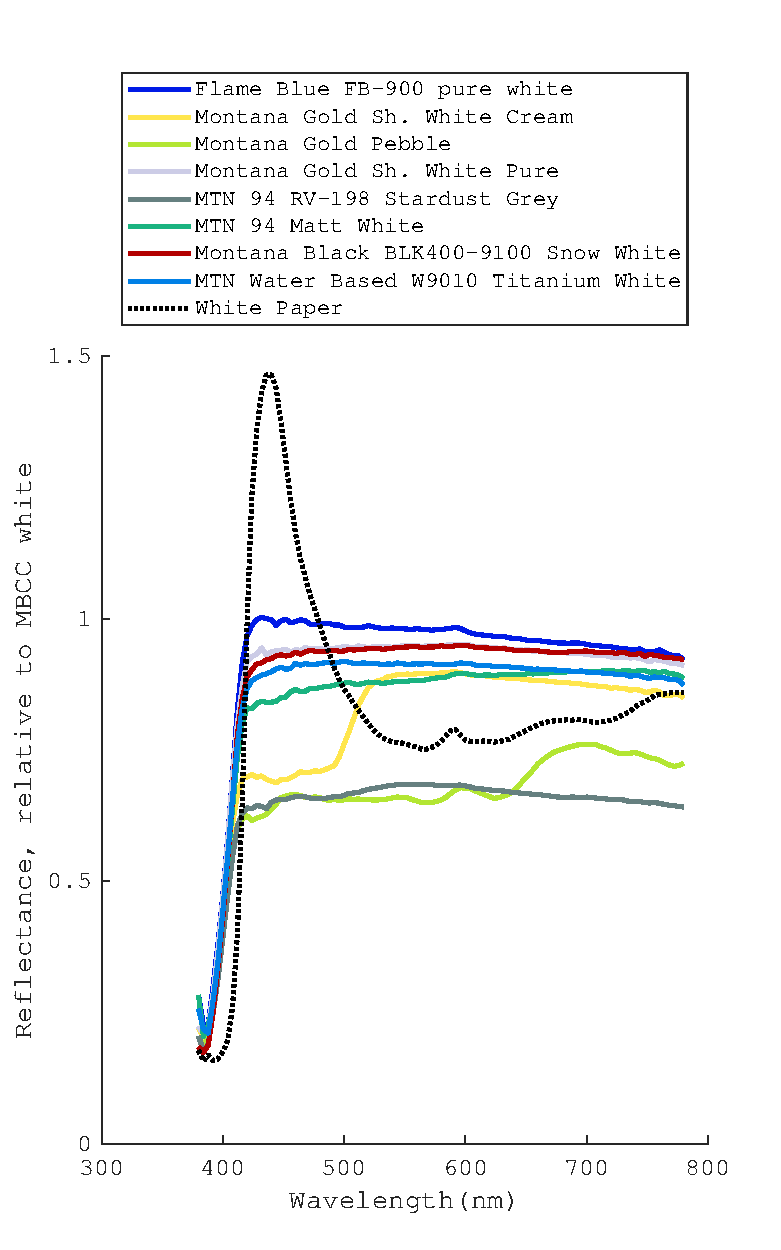
\includegraphics[max width=\textwidth]{figs/SmallSphere/VisualiseSPDs_result.pdf}
\caption{The \glspl{SRF} of the 8 tested paints (relative to the white patch of a MacBeth Colour Checker card, which is known to be very uniform in spectral reflectance) with an additional measurement of a piece of white office paper to demonstrate how a fluorescent additive might appear.}
\label{fig:spray}
\end{figure}


\subsection{The screen}

The screen was offset by roughly 150mm through a short black paper tube in order to limit the interference (either way) between the screen illuminant and the sphere illuminant. 

%Primaries
%Gamut

\subsubsection{Characterisation}

Following the disappointment of the data collection phase of the Large Sphere experiment, two separate characterisation procedures were performed, one before and one after every set of observations (in addition to the monitoring of illumination inside the sphere).

The first characterisation routine is rather standard - a spectral measurement of the display primaries followed by a ramping through pixel space for each display channel from zero output to maximum output\footnote{Controlled by the script available at \url{https://github.com/da5nsy/Small-Sphere/blob/5c6af38c5036a4c0a328a9854427ae8e851e84fd/Hardware\%20Specs/PR650\%20Screen\%20Measurements/PR650displaycharacterisation_DG.m}}. This was only measured for the small portion of the screen which would be used during experiments.

The second calibration procedure attempted to include any issues which may arise due to the specific specification method used within the experiment. A very minor amendment was made to a copy of the main experimental script, such that it only included 3 repeats rather than 30. %haven't introduced this yet
This script was run in exactly the same way that the main experimental script would be run, except that the observer was replaced by our \gls{PR650}, and no effort was made to select neutral points. In this way, a random selection of points were recorded, and through comparison with the recorded `responses', it could be seen whether there was any discrepancy between what we thought was being displayed on the screen and what was actually being displayed on the screen.
% demo?

\subsection{The LED rig}

50 LEDs, mounted in a breadboard, were controlled by an Arduini Uno.

\begin{itemize}
    \item 20: Bivar UV5TZ-400-15
    \item 10: Cree C503B-BCS-CV0Z0461
    \item 10: Cree C503B-AAS-CA0C0251-015
    \item 10: Cree C503B-RAS-CY0B0AA2
\end{itemize}
\end{item}

%UNOPENED 
%810-6705 C503D-WAN-CCbEb151
%810-6636 C503B-AAN-CY0B0251
%810-0492 C503B-BCN-CV0Z0461

These LEDs were chosen such that a \dots

% (metamer setting)
% The controllers 
% The code
% Characterisation / ongoing measurement

\subsection{Observer task}
% Observers were...
% Initial metamer setting
% Achromatic selections


\section{Results}


\section{Discussion}
% Assumptions
